In questa sezione vengono presentati, per ogni macro-fase di progetto, le ore preventivate di impiego per i ruoli coinvolti.

\noindent Occorre ricordare che le macro-fasi di \textbf{Analisi} e \textbf{Analisi di Dettaglio} non sono a carico del committente e quindi non saranno considerate nel computo delle ore totali da retribuire, ma verranno riportate ugualmente per dare un'immagine di insieme.

\subsection{Analisi}
In questa macro-fase, le ore ripartite tra i ruoli ed i conseguenti costi sono evidenziati dalla seguente tabella:

\begin{table}[h]
\centering
\begin{tabular}{|l|c|c|}
	\toprule
	\textbf{Ruolo} & \textbf{Ore per ruolo} & \textbf{Costo per ruolo} \\
			
	\midrule
	Responsabile di Progetto & 17 & 510 \\
	Amministratore di Progetto & 26 & 520 \\ 
	Analista & 50 & 1250 \\
	Progettista & & \\
	Programmatore & & \\
	Verificatore & 37 & 555 \\
	\midrule
	\textbf{Totale} & 130 & 2835 \\
				
	\bottomrule
\end{tabular}
\caption{Costo per ruolo, Analisi}
\end{table}

\noindent Il seguente grafico illustra come ciascun ruolo abbia influito sul totale delle ore di questa macro-fase:

\def\angle{0}
\def\radius{3}
\def\cyclelist{{"blue","red","yellow","green"}}
\newcount\cyclecount \cyclecount=-1
\newcount\ind \ind=-1
\begin{figure}[h]
\centering
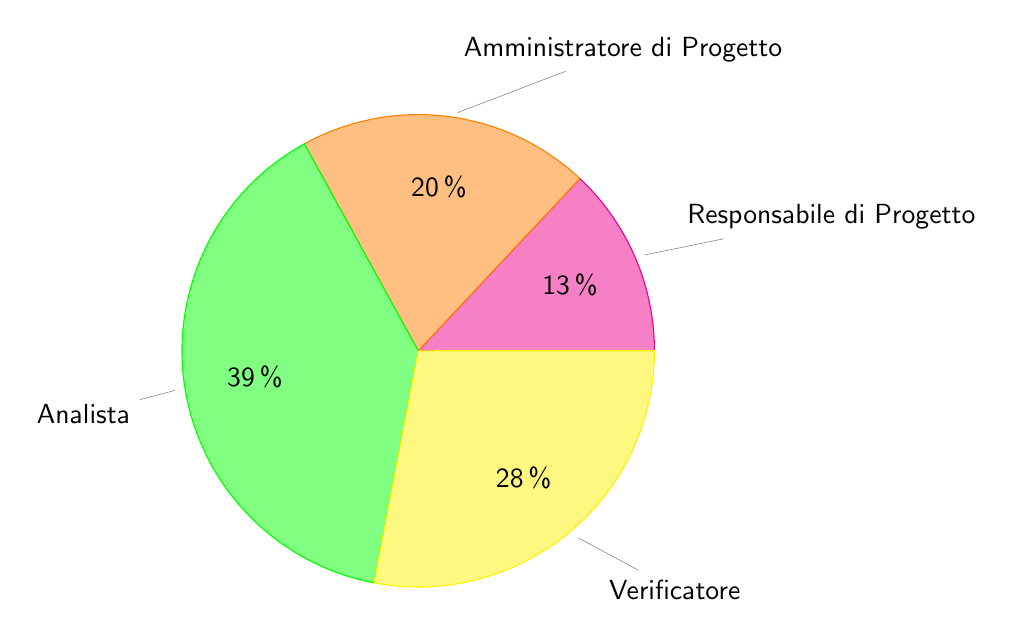
\begin{tikzpicture}[nodes = {font=\sffamily}]
\foreach \percent/\name in {
	13/Responsabile di Progetto,
	20/Amministratore di Progetto,
	39/Analista,
	28/Verificatore
} {
\ifx\percent\empty\else               % If \percent is empty, do nothing
\global\advance\cyclecount by 1     % Advance cyclecount
\global\advance\ind by 1            % Advance list index
\ifnum3<\cyclecount                 % If cyclecount is larger than list
\global\cyclecount=0              %   reset cyclecount and
\global\ind=0                     %   reset list index
\fi
\pgfmathparse{\cyclelist[\the\ind]} % Get color from cycle list
\edef\color{\pgfmathresult}         %   and store as \color
% Draw angle and set labels
\draw[fill={\color!50},draw={\color}] (0,0) -- (\angle:\radius)
arc (\angle:\angle+\percent*3.6:\radius) -- cycle;
\node at (\angle+0.5*\percent*3.6:0.7*\radius) {\percent\,\%};
\node[pin=\angle+0.5*\percent*3.6:\name]
at (\angle+0.5*\percent*3.6:\radius) {};
\pgfmathparse{\angle+\percent*3.6}  % Advance angle
\xdef\angle{\pgfmathresult}         %   and store in \angle
\fi
};
\end{tikzpicture}
\caption{Ore per ruoli, Analisi}
\end{figure}
\newpage

\noindent Il seguente grafico illustra come ciascun ruolo abbia influito sul totale dei costi di questa macro-fase:

\begin{figure}[h]
\centering
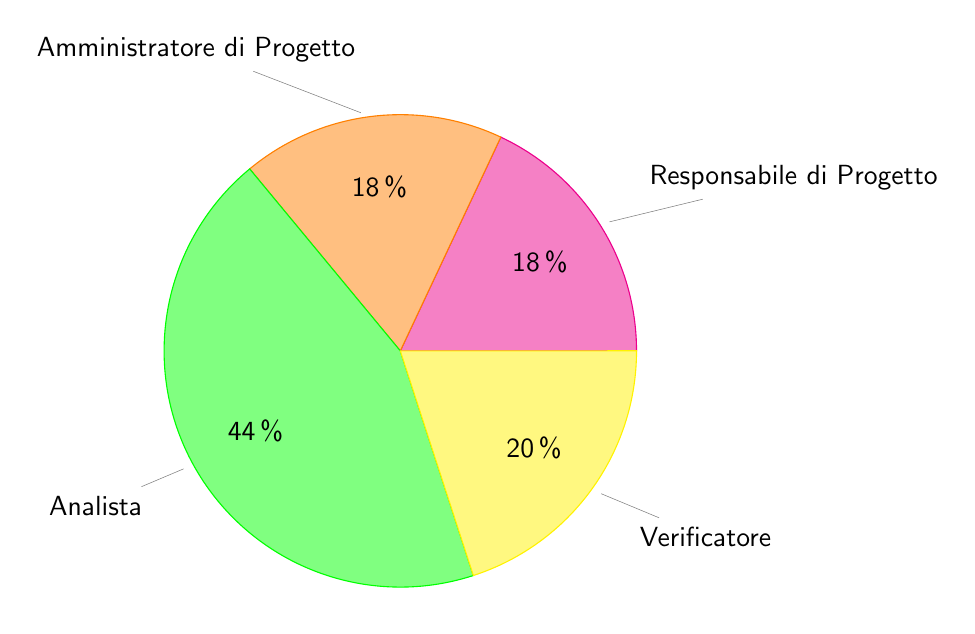
\begin{tikzpicture}[nodes = {font=\sffamily}]
	\foreach \percent/\name in {
		18/Responsabile di Progetto,
		18/Amministratore di Progetto,
		44/Analista,
		20/Verificatore
	} {
		\ifx\percent\empty\else               % If \percent is empty, do nothing
		\global\advance\cyclecount by 1     % Advance cyclecount
		\global\advance\ind by 1            % Advance list index
		\ifnum3<\cyclecount                 % If cyclecount is larger than list
		\global\cyclecount=0              %   reset cyclecount and
		\global\ind=0                     %   reset list index
		\fi
		\pgfmathparse{\cyclelist[\the\ind]} % Get color from cycle list
		\edef\color{\pgfmathresult}         %   and store as \color
		% Draw angle and set labels
		\draw[fill={\color!50},draw={\color}] (0,0) -- (\angle:\radius)
		arc (\angle:\angle+\percent*3.6:\radius) -- cycle;
		\node at (\angle+0.5*\percent*3.6:0.7*\radius) {\percent\,\%};
		\node[pin=\angle+0.5*\percent*3.6:\name]
		at (\angle+0.5*\percent*3.6:\radius) {};
		\pgfmathparse{\angle+\percent*3.6}  % Advance angle
		\xdef\angle{\pgfmathresult}         %   and store in \angle
		\fi
	};
\end{tikzpicture}
\caption{Costo per ruoli, Analisi}
\end{figure}

\subsection{Analisi di Dettaglio}
In questa macro-fase, le ore ripartite tra i ruoli ed i conseguenti costi sono evidenziati dalla seguente tabella:

\begin{table}[h]
\centering
\begin{tabular}{|l|c|c|}
	\toprule
	\textbf{Ruolo} & \textbf{Ore per ruolo} & \textbf{Costo per ruolo} \\
		
	\midrule
	Responsabile di Progetto & 4 & 120 \\
	Amministratore di Progetto & 4 & 80 \\ 
	Analista & 18 & 450 \\
	Progettista & & \\
	Programmatore & & \\
	Verificatore & 12 & 180 \\
	\midrule
	\textbf{Totale} & 38 & 830 \\
		
	\bottomrule
\end{tabular}
\caption{Costo per ruolo, Analisi di Dettaglio}
\end{table}

\newpage
\noindent I seguenti grafici illustrano rispettivamente come ciascun ruolo abbia influito sul totale delle ore e dei costi di questa macro-fase:

\begin{figure}[h]
\centering
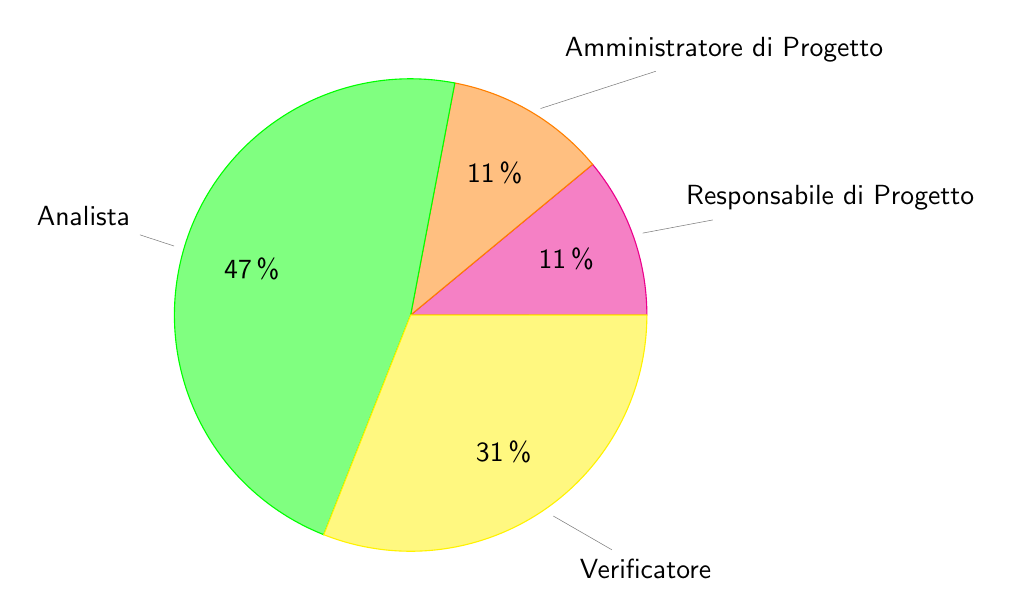
\begin{tikzpicture}[nodes = {font=\sffamily}]
	\foreach \percent/\name in {
		11/Responsabile di Progetto,
		11/Amministratore di Progetto,
		47/Analista,
		31/Verificatore
	} {
	\ifx\percent\empty\else               % If \percent is empty, do nothing
	\global\advance\cyclecount by 1     % Advance cyclecount
	\global\advance\ind by 1            % Advance list index
	\ifnum3<\cyclecount                 % If cyclecount is larger than list
	\global\cyclecount=0              %   reset cyclecount and
	\global\ind=0                     %   reset list index
	\fi
	\pgfmathparse{\cyclelist[\the\ind]} % Get color from cycle list
	\edef\color{\pgfmathresult}         %   and store as \color
	% Draw angle and set labels
	\draw[fill={\color!50},draw={\color}] (0,0) -- (\angle:\radius)
	arc (\angle:\angle+\percent*3.6:\radius) -- cycle;
	\node at (\angle+0.5*\percent*3.6:0.7*\radius) {\percent\,\%};
	\node[pin=\angle+0.5*\percent*3.6:\name]
	at (\angle+0.5*\percent*3.6:\radius) {};
	\pgfmathparse{\angle+\percent*3.6}  % Advance angle
	\xdef\angle{\pgfmathresult}         %   and store in \angle
	\fi
};
\end{tikzpicture}
\caption{Ore per ruoli, Analisi di Dettaglio}
\end{figure}

\begin{figure}[h]
\centering
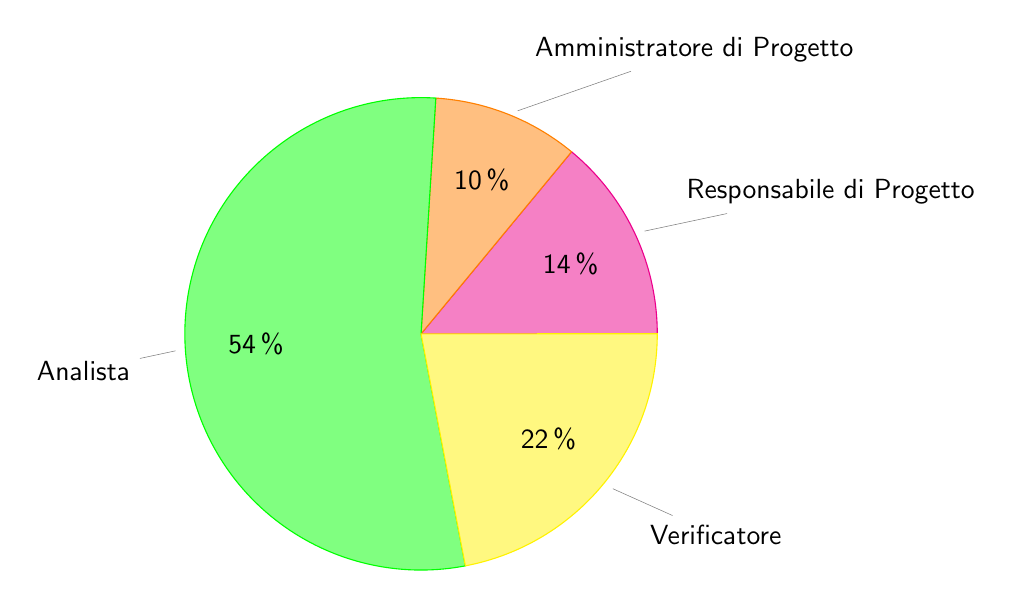
\begin{tikzpicture}[nodes = {font=\sffamily}]
	\foreach \percent/\name in {
		14/Responsabile di Progetto,
		10/Amministratore di Progetto,
		54/Analista,
		22/Verificatore
	} {
	\ifx\percent\empty\else               % If \percent is empty, do nothing
	\global\advance\cyclecount by 1     % Advance cyclecount
	\global\advance\ind by 1            % Advance list index
	\ifnum3<\cyclecount                 % If cyclecount is larger than list
	\global\cyclecount=0              %   reset cyclecount and
	\global\ind=0                     %   reset list index
	\fi
	\pgfmathparse{\cyclelist[\the\ind]} % Get color from cycle list
	\edef\color{\pgfmathresult}         %   and store as \color
	% Draw angle and set labels
	\draw[fill={\color!50},draw={\color}] (0,0) -- (\angle:\radius)
	arc (\angle:\angle+\percent*3.6:\radius) -- cycle;
	\node at (\angle+0.5*\percent*3.6:0.7*\radius) {\percent\,\%};
	\node[pin=\angle+0.5*\percent*3.6:\name]
	at (\angle+0.5*\percent*3.6:\radius) {};
	\pgfmathparse{\angle+\percent*3.6}  % Advance angle
	\xdef\angle{\pgfmathresult}         %   and store in \angle
	\fi
};
\end{tikzpicture}
\caption{Costo per ruoli, Analisi di Dettaglio}
\end{figure}
\newpage
\subsection{Progettazione Architetturale}
In questa macro-fase, le ore ripartite tra i ruoli ed i conseguenti costi sono evidenziati dalla seguente tabella:

\begin{table}[h]
\centering
\begin{tabular}{|l|c|c|}
	\toprule
	\textbf{Ruolo} & \textbf{Ore per ruolo} & \textbf{Costo per ruolo} \\
		
	\midrule
	Responsabile di Progetto & 5 & 150 \\
	Amministratore di Progetto & 5 & 100 \\ 
	Analista & 16 & 400 \\
	Progettista & 100 & 2200 \\
	Programmatore & & \\
	Verificatore & 41 & 615 \\
	\midrule
	\textbf{Totale} & 167 & 3465 \\
	
	\bottomrule
\end{tabular}
\caption{Costo per ruolo, Progettazione Architetturale}
\end{table}

\noindent Il seguente grafico illustra come ciascun ruolo abbia influito sul totale delle ore di questa macro-fase:

\def\cyclelist{{"red","yellow","magenta","green","blue"}}
\begin{figure}[h]
\centering
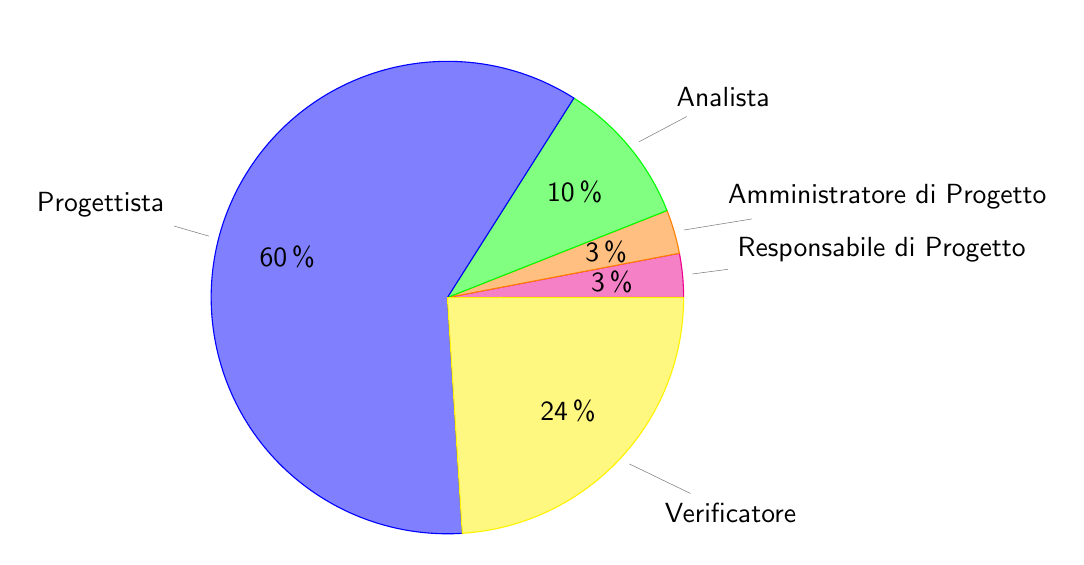
\begin{tikzpicture}[nodes = {font=\sffamily}]
	\foreach \percent/\name in {
		3/Responsabile di Progetto,
		3/Amministratore di Progetto,
		10/Analista,
		60/Progettista,
		24/Verificatore
	} {
	\ifx\percent\empty\else               % If \percent is empty, do nothing
	\global\advance\cyclecount by 1     % Advance cyclecount
	\global\advance\ind by 1            % Advance list index
	\ifnum4<\cyclecount                 % If cyclecount is larger than list
	\global\cyclecount=0              %   reset cyclecount and
	\global\ind=0                     %   reset list index
	\fi
	\pgfmathparse{\cyclelist[\the\ind]} % Get color from cycle list
	\edef\color{\pgfmathresult}         %   and store as \color
	% Draw angle and set labels
	\draw[fill={\color!50},draw={\color}] (0,0) -- (\angle:\radius)
	arc (\angle:\angle+\percent*3.6:\radius) -- cycle;
	\node at (\angle+0.5*\percent*3.6:0.7*\radius) {\percent\,\%};
	\node[pin=\angle+0.5*\percent*3.6:\name]
	at (\angle+0.5*\percent*3.6:\radius) {};
	\pgfmathparse{\angle+\percent*3.6}  % Advance angle
	\xdef\angle{\pgfmathresult}         %   and store in \angle
	\fi
};
\end{tikzpicture}
\caption{Ore per ruoli, Progettazione Architetturale}
\end{figure}
\newpage

\noindent Il seguente grafico illustra come ciascun ruolo abbia influito sul totale dei costi di questa macro-fase:

\begin{figure}[h]
\centering
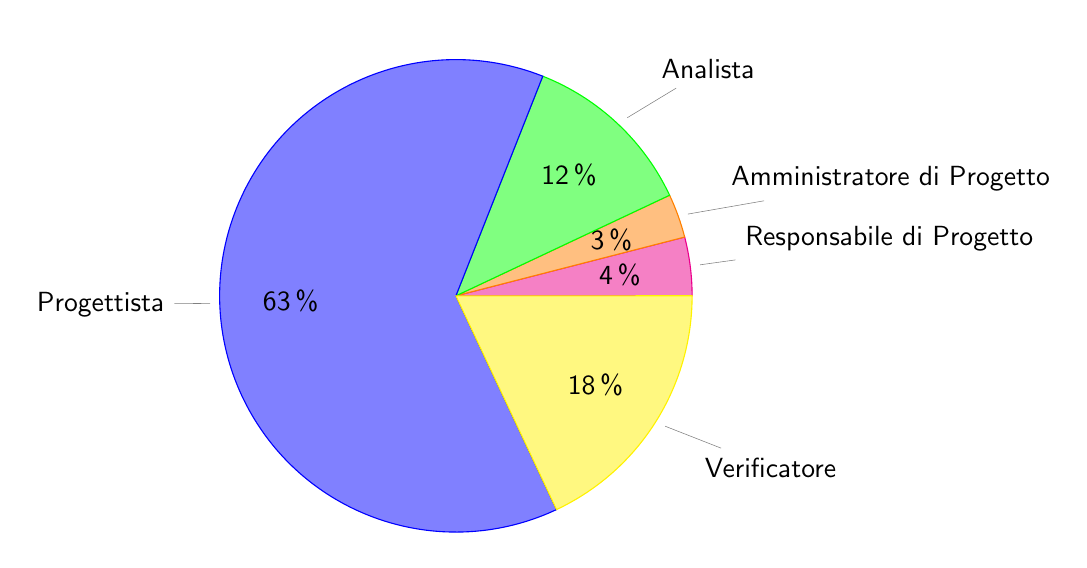
\begin{tikzpicture}[nodes = {font=\sffamily}]
	\foreach \percent/\name in {
		4/Responsabile di Progetto,
		3/Amministratore di Progetto,
		12/Analista,
		63/Progettista,
		18/Verificatore
	} {
	\ifx\percent\empty\else               % If \percent is empty, do nothing
	\global\advance\cyclecount by 1     % Advance cyclecount
	\global\advance\ind by 1            % Advance list index
	\ifnum4<\cyclecount                 % If cyclecount is larger than list
	\global\cyclecount=0              %   reset cyclecount and
	\global\ind=0                     %   reset list index
	\fi
	\pgfmathparse{\cyclelist[\the\ind]} % Get color from cycle list
	\edef\color{\pgfmathresult}         %   and store as \color
	% Draw angle and set labels
	\draw[fill={\color!50},draw={\color}] (0,0) -- (\angle:\radius)
	arc (\angle:\angle+\percent*3.6:\radius) -- cycle;
	\node at (\angle+0.5*\percent*3.6:0.7*\radius) {\percent\,\%};
	\node[pin=\angle+0.5*\percent*3.6:\name]
	at (\angle+0.5*\percent*3.6:\radius) {};
	\pgfmathparse{\angle+\percent*3.6}  % Advance angle
	\xdef\angle{\pgfmathresult}         %   and store in \angle
	\fi
};
\end{tikzpicture}
\caption{Costo per ruoli, Progettazione Architetturale}
\end{figure}

\subsection{Progettazione di Dettaglio e Codifica}
In questa macro-fase, le ore ripartite tra i ruoli ed i conseguenti costi sono evidenziati dalla seguente tabella:

\begin{table}[h]
\centering
\begin{tabular}{|l|c|c|}
	\toprule
	\textbf{Ruolo} & \textbf{Ore per ruolo} & \textbf{Costo per ruolo} \\
		
	\midrule
	Responsabile di Progetto & 4 & 120 \\
	Amministratore di Progetto & 4 & 80 \\ 
	Analista & 4 & 100 \\
	Progettista & 64 & 1408 \\
	Programmatore & 174 & 2610 \\
	Verificatore & 66 & 990 \\
	\midrule
	\textbf{Totale} & 316 & 5308 \\
	
	\bottomrule
\end{tabular}
\caption{Costo per ruolo, Progettazione di Dettaglio e Codifica}
\end{table}

\newpage
\noindent I seguenti grafici illustrano rispettivamente come ciascun ruolo abbia influito sul totale delle ore e dei costi di questa macro-fase:
\def\cyclelist{{"yellow","magenta","orange","green","blue","red"}}
\begin{figure}[h]
\centering
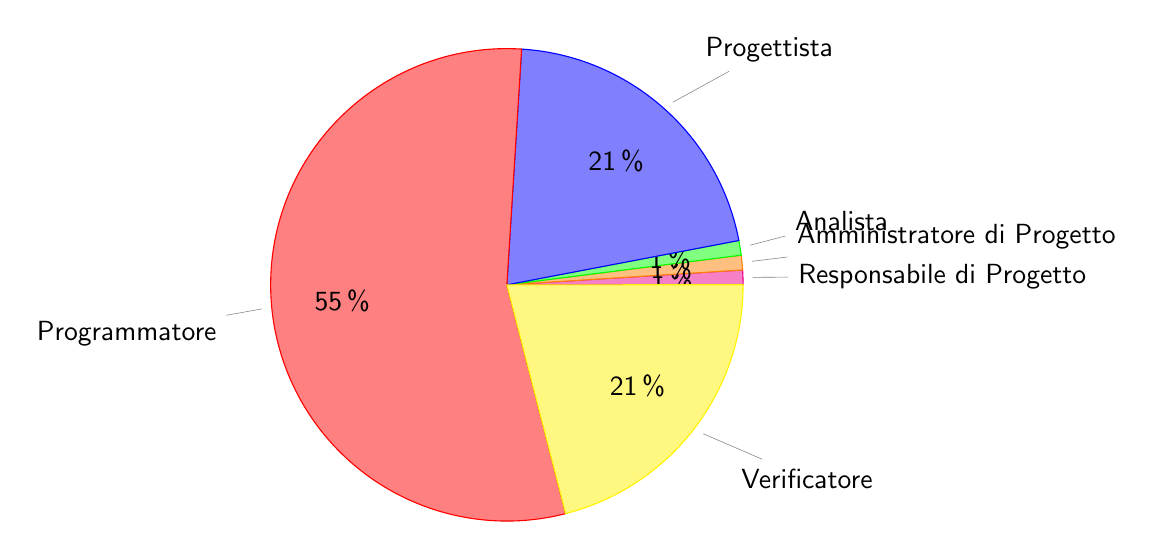
\begin{tikzpicture}[nodes = {font=\sffamily}]
	\foreach \percent/\name in {
		1/Responsabile di Progetto,
		1/Amministratore di Progetto,
		1/Analista,
		21/Progettista,
		55/Programmatore,
		21/Verificatore
	} {
	\ifx\percent\empty\else               % If \percent is empty, do nothing
	\global\advance\cyclecount by 1     % Advance cyclecount
	\global\advance\ind by 1            % Advance list index
	\ifnum5<\cyclecount                 % If cyclecount is larger than list
	\global\cyclecount=0              %   reset cyclecount and
	\global\ind=0                     %   reset list index
	\fi
	\pgfmathparse{\cyclelist[\the\ind]} % Get color from cycle list
	\edef\color{\pgfmathresult}         %   and store as \color
	% Draw angle and set labels
	\draw[fill={\color!50},draw={\color}] (0,0) -- (\angle:\radius)
	arc (\angle:\angle+\percent*3.6:\radius) -- cycle;
	\node at (\angle+0.5*\percent*3.6:0.7*\radius) {\percent\,\%};
	\node[pin=\angle+0.5*\percent*3.6:\name]
	at (\angle+0.5*\percent*3.6:\radius) {};
	\pgfmathparse{\angle+\percent*3.6}  % Advance angle
	\xdef\angle{\pgfmathresult}         %   and store in \angle
	\fi
};
\end{tikzpicture}
\caption{Ore per ruoli, Progettazione di Dettaglio e Codifica}
\end{figure}

\begin{figure}[h]
\centering
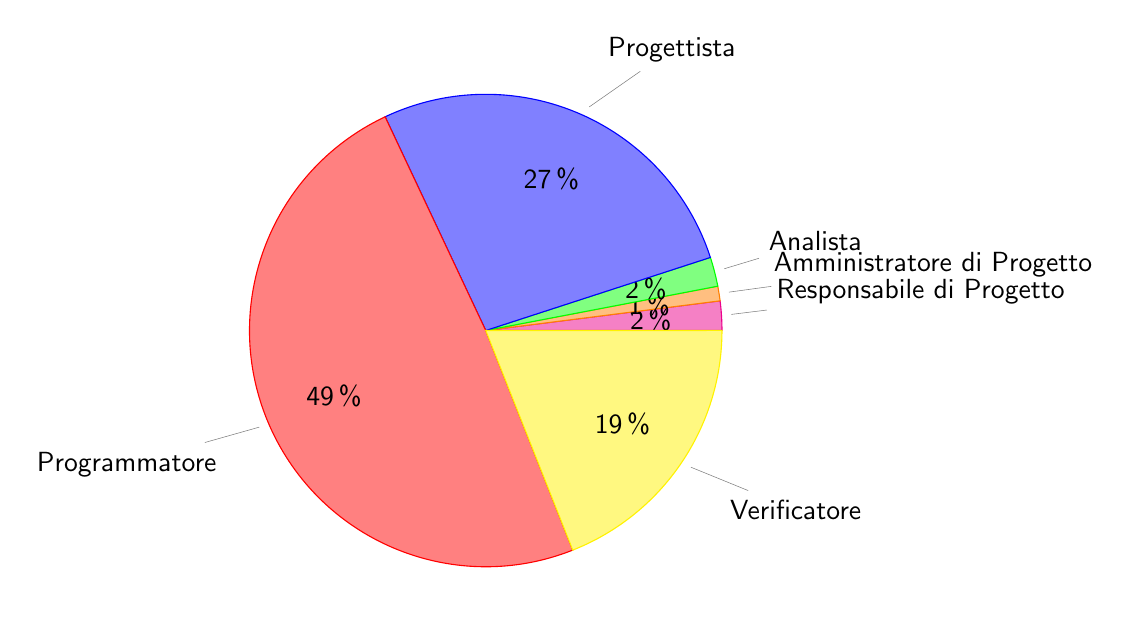
\begin{tikzpicture}[nodes = {font=\sffamily}]
	\foreach \percent/\name in {
		2/Responsabile di Progetto,
		1/Amministratore di Progetto,
		2/Analista,
		27/Progettista,
		49/Programmatore,
		19/Verificatore
	} {
	\ifx\percent\empty\else               % If \percent is empty, do nothing
	\global\advance\cyclecount by 1     % Advance cyclecount
	\global\advance\ind by 1            % Advance list index
	\ifnum5<\cyclecount                 % If cyclecount is larger than list
	\global\cyclecount=0              %   reset cyclecount and
	\global\ind=0                     %   reset list index
	\fi
	\pgfmathparse{\cyclelist[\the\ind]} % Get color from cycle list
	\edef\color{\pgfmathresult}         %   and store as \color
	% Draw angle and set labels
	\draw[fill={\color!50},draw={\color}] (0,0) -- (\angle:\radius)
	arc (\angle:\angle+\percent*3.6:\radius) -- cycle;
	\node at (\angle+0.5*\percent*3.6:0.7*\radius) {\percent\,\%};
	\node[pin=\angle+0.5*\percent*3.6:\name]
	at (\angle+0.5*\percent*3.6:\radius) {};
	\pgfmathparse{\angle+\percent*3.6}  % Advance angle
	\xdef\angle{\pgfmathresult}         %   and store in \angle
	\fi
};
\end{tikzpicture}
\caption{Costo per ruoli, Progettazione di Dettaglio e Codifica}
\end{figure}

\newpage
\subsection{Verifica e Validazione}
In questa macro-fase, le ore ripartite tra i ruoli ed i conseguenti costi sono evidenziati dalla seguente tabella:

\begin{table}[h]
\centering
\begin{tabular}{|l|c|c|}
	\toprule
	\textbf{Ruolo} & \textbf{Ore per ruolo} & \textbf{Costo per ruolo} \\
		
	\midrule
	Responsabile di Progetto & 8 & 240 \\
	Amministratore di Progetto & 8 & 160 \\ 
	Analista & 8 & 200 \\
	Progettista & 25 & 550 \\
	Programmatore & 16 & 240 \\
	Verificatore & 82 & 1230 \\
	\midrule
	\textbf{Totale} & 147 & 2620 \\
		
	\bottomrule
\end{tabular}
\caption{Costo per ruolo, Verifica e Validazione}
\end{table}

\noindent Il seguente grafico illustra come ciascun ruolo abbia influito sul totale delle ore di questa macro-fase:

\begin{figure}[h]
\centering
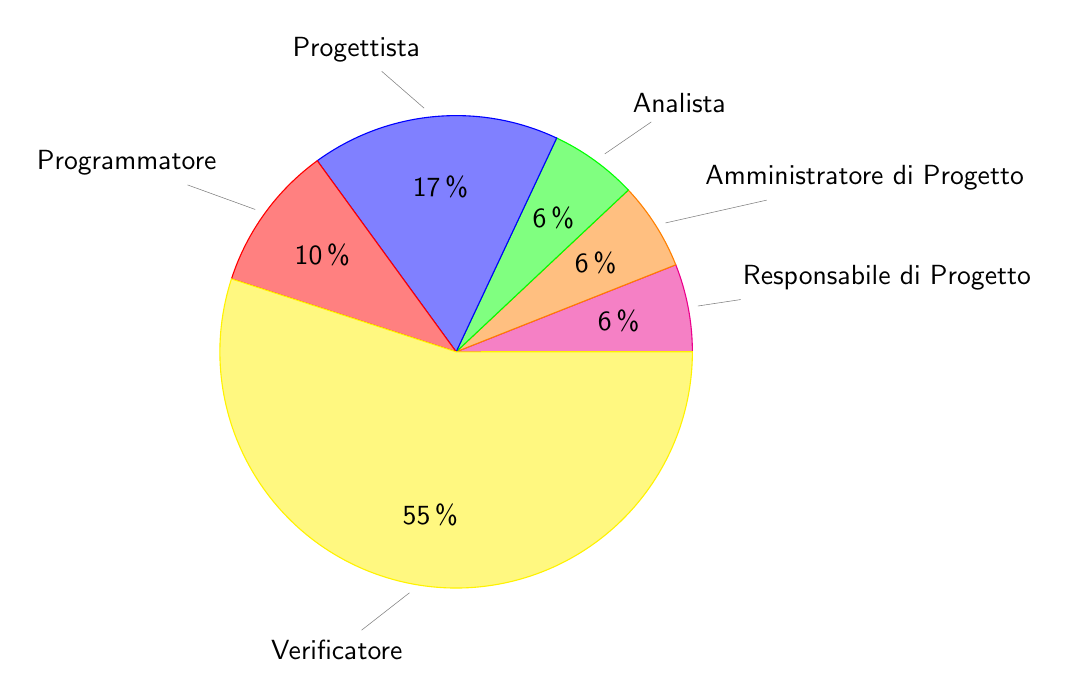
\begin{tikzpicture}[nodes = {font=\sffamily}]
	\foreach \percent/\name in {
		6/Responsabile di Progetto,
		6/Amministratore di Progetto,
		6/Analista,
		17/Progettista,
		10/Programmatore,
		55/Verificatore
	} {
	\ifx\percent\empty\else               % If \percent is empty, do nothing
	\global\advance\cyclecount by 1     % Advance cyclecount
	\global\advance\ind by 1            % Advance list index
	\ifnum5<\cyclecount                 % If cyclecount is larger than list
	\global\cyclecount=0              %   reset cyclecount and
	\global\ind=0                     %   reset list index
	\fi
	\pgfmathparse{\cyclelist[\the\ind]} % Get color from cycle list
	\edef\color{\pgfmathresult}         %   and store as \color
	% Draw angle and set labels
	\draw[fill={\color!50},draw={\color}] (0,0) -- (\angle:\radius)
	arc (\angle:\angle+\percent*3.6:\radius) -- cycle;
	\node at (\angle+0.5*\percent*3.6:0.7*\radius) {\percent\,\%};
	\node[pin=\angle+0.5*\percent*3.6:\name]
	at (\angle+0.5*\percent*3.6:\radius) {};
	\pgfmathparse{\angle+\percent*3.6}  % Advance angle
	\xdef\angle{\pgfmathresult}         %   and store in \angle
	\fi
};
\end{tikzpicture}
\caption{Ore per ruoli, Verifica e Validazione}
\end{figure}

\newpage
\noindent Il seguente grafico illustra come ciascun ruolo abbia influito sul totale dei costi di questa macro-fase:

\begin{figure}[h]
\centering
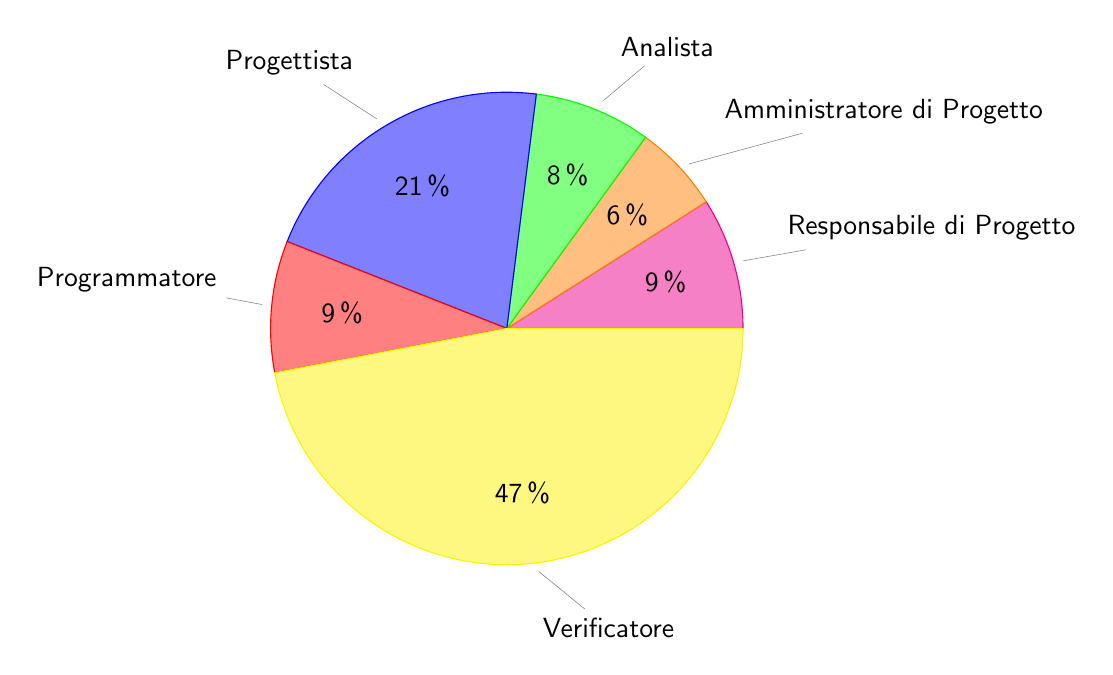
\begin{tikzpicture}[nodes = {font=\sffamily}]
	\foreach \percent/\name in {
		9/Responsabile di Progetto,
		6/Amministratore di Progetto,
		8/Analista,
		21/Progettista,
		9/Programmatore,
		47/Verificatore
	} {
	\ifx\percent\empty\else               % If \percent is empty, do nothing
	\global\advance\cyclecount by 1     % Advance cyclecount
	\global\advance\ind by 1            % Advance list index
	\ifnum5<\cyclecount                 % If cyclecount is larger than list
	\global\cyclecount=0              %   reset cyclecount and
	\global\ind=0                     %   reset list index
	\fi
	\pgfmathparse{\cyclelist[\the\ind]} % Get color from cycle list
	\edef\color{\pgfmathresult}         %   and store as \color
	% Draw angle and set labels
	\draw[fill={\color!50},draw={\color}] (0,0) -- (\angle:\radius)
	arc (\angle:\angle+\percent*3.6:\radius) -- cycle;
	\node at (\angle+0.5*\percent*3.6:0.7*\radius) {\percent\,\%};
	\node[pin=\angle+0.5*\percent*3.6:\name]
	at (\angle+0.5*\percent*3.6:\radius) {};
	\pgfmathparse{\angle+\percent*3.6}  % Advance angle
	\xdef\angle{\pgfmathresult}         %   and store in \angle
	\fi
};
\end{tikzpicture}
\caption{Costo per ruoli, Verifica e Validazione}
\end{figure}

\subsection{Totale}
\subsubsection{Ore totali e rendicontate}
Le ore totali previste per la realizzazione dell'intero progetto, suddivise in ore totali e rendicontate, ed i conseguenti costi sono riportate nella seguente tabella:

\begin{table}[h]
\centering
\begin{tabular}{|l|l|c|c|c|c|c|c|c|}
	\toprule
	\textbf{Ruolo} & & \textbf{Ore per ruolo} & \textbf{Costo per ruolo} \\
		
	\midrule
	\multirow{2}*{Responsabile di Progetto} & Totale & 38 & 1140 \\
												& Rendicontanto & 17 & 510 \\
    \midrule
	\multirow{2}*{Amministratore di Progetto} & Totale & 47 & 940 \\
												  & Rendicontanto & 17 & 340 \\ 
	\midrule
	\multirow{2}*{Analista} & Totale & 96 & 2400 \\
								& Rendicontanto & 28 & 700 \\
	\midrule
	\multirow{2}*{Progettista} & Totale & 189 & 4158 \\
								   & Rendicontanto & 189 & 4158 \\
	\midrule
	\multirow{2}*{Programmatore} & Totale & 190 & 2850 \\
									 & Rendicontanto & 190 & 2850 \\ 
	\midrule
	\multirow{2}*{Verificatore} & Totale & 238 & 3570 \\
									& Rendicontanto & 189 & 2835 \\
	\midrule							
	\multirow{2}*{} & Totale & 798 & 15058 \\
						& Rendicontanto & \textbf{630} & \textbf{11393} \\
	\bottomrule
		
\end{tabular}
\caption{Ore a componente per ruolo, Totali e Rendicontate}
\label{tab2}
\end{table}

\newpage
\noindent I seguenti grafici illustrano, rispettivamente, l'incidenza di ciascun ruolo su orari e costi totali del progetto \PROGETTO:

\begin{figure}[h]
\centering
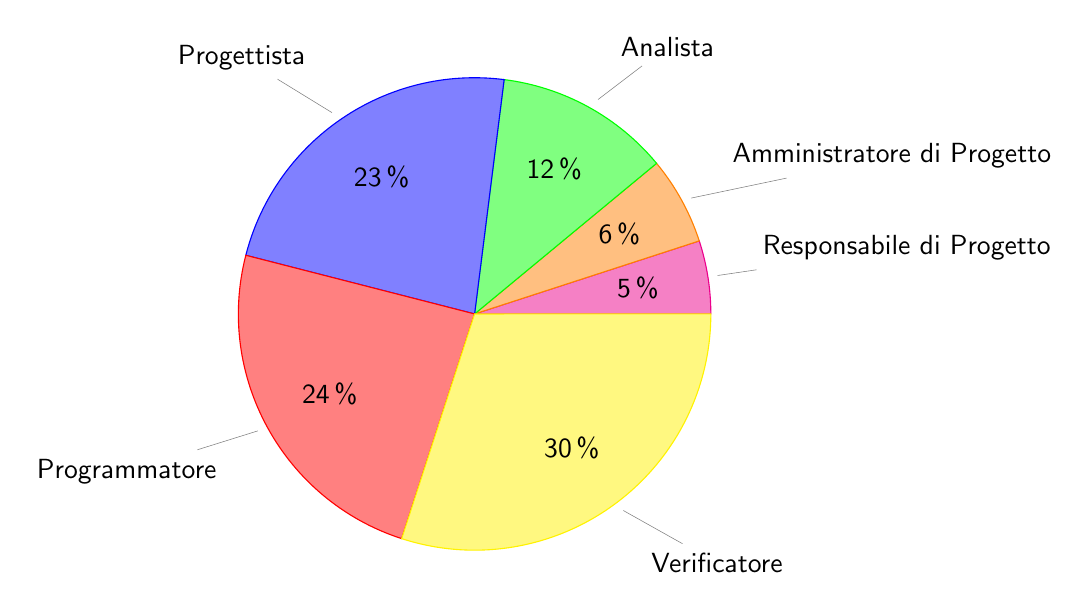
\begin{tikzpicture}[nodes = {font=\sffamily}]
	\foreach \percent/\name in {
		5/Responsabile di Progetto,
		6/Amministratore di Progetto,
		12/Analista,
		23/Progettista,
		24/Programmatore,
		30/Verificatore
	} {
	\ifx\percent\empty\else               % If \percent is empty, do nothing
	\global\advance\cyclecount by 1     % Advance cyclecount
	\global\advance\ind by 1            % Advance list index
	\ifnum5<\cyclecount                 % If cyclecount is larger than list
	\global\cyclecount=0              %   reset cyclecount and
	\global\ind=0                     %   reset list index
	\fi
	\pgfmathparse{\cyclelist[\the\ind]} % Get color from cycle list
	\edef\color{\pgfmathresult}         %   and store as \color
	% Draw angle and set labels
	\draw[fill={\color!50},draw={\color}] (0,0) -- (\angle:\radius)
	arc (\angle:\angle+\percent*3.6:\radius) -- cycle;
	\node at (\angle+0.5*\percent*3.6:0.7*\radius) {\percent\,\%};
	\node[pin=\angle+0.5*\percent*3.6:\name]
	at (\angle+0.5*\percent*3.6:\radius) {};
	\pgfmathparse{\angle+\percent*3.6}  % Advance angle
	\xdef\angle{\pgfmathresult}         %   and store in \angle
	\fi
};
\end{tikzpicture}
\caption{Ore totali per ruoli}
\end{figure}

\begin{figure}[h]
\centering
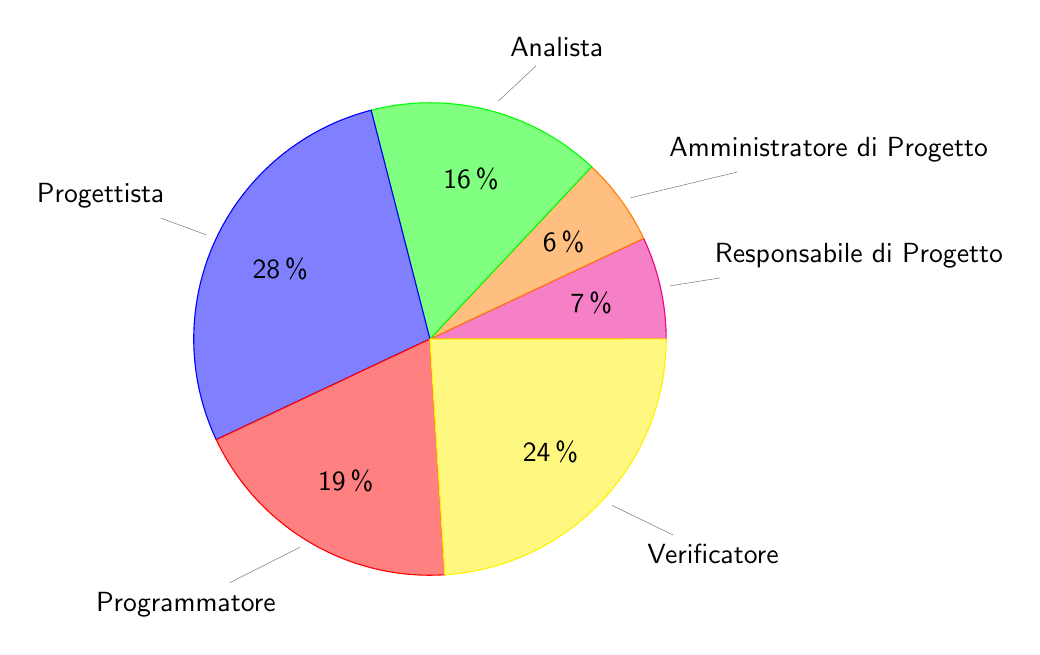
\begin{tikzpicture}[nodes = {font=\sffamily}]
	\foreach \percent/\name in {
		7/Responsabile di Progetto,
		6/Amministratore di Progetto,
		16/Analista,
		28/Progettista,
		19/Programmatore,
		24/Verificatore
	} {
	\ifx\percent\empty\else               % If \percent is empty, do nothing
	\global\advance\cyclecount by 1     % Advance cyclecount
	\global\advance\ind by 1            % Advance list index
	\ifnum5<\cyclecount                 % If cyclecount is larger than list
	\global\cyclecount=0              %   reset cyclecount and
	\global\ind=0                     %   reset list index
	\fi
	\pgfmathparse{\cyclelist[\the\ind]} % Get color from cycle list
	\edef\color{\pgfmathresult}         %   and store as \color
	% Draw angle and set labels
	\draw[fill={\color!50},draw={\color}] (0,0) -- (\angle:\radius)
	arc (\angle:\angle+\percent*3.6:\radius) -- cycle;
	\node at (\angle+0.5*\percent*3.6:0.7*\radius) {\percent\,\%};
	\node[pin=\angle+0.5*\percent*3.6:\name]
	at (\angle+0.5*\percent*3.6:\radius) {};
	\pgfmathparse{\angle+\percent*3.6}  % Advance angle
	\xdef\angle{\pgfmathresult}         %   and store in \angle
	\fi
};
\end{tikzpicture}
\caption{Costi totali per ruoli}
\end{figure}

\newpage
\noindent I seguenti grafici illustrano, rispettivamente, l'incidenza di ciascun ruolo su orari e costi rendicontati del progetto \PROGETTO:

\begin{figure}[h]
\centering
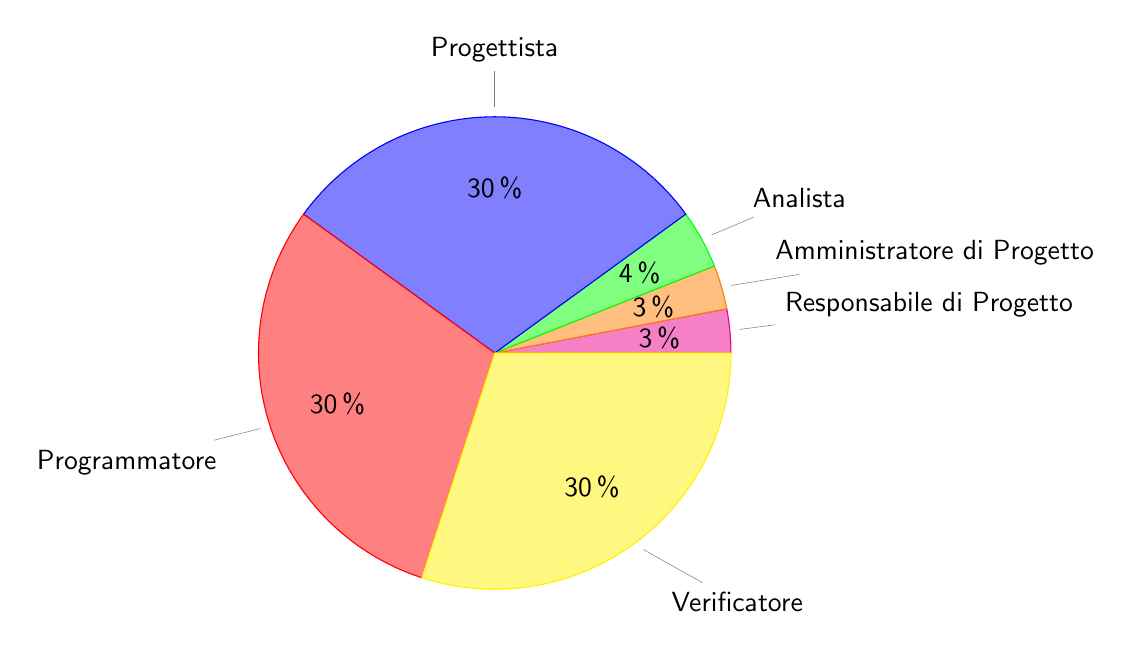
\begin{tikzpicture}[nodes = {font=\sffamily}]
	\foreach \percent/\name in {
		3/Responsabile di Progetto,
		3/Amministratore di Progetto,
		4/Analista,
		30/Progettista,
		30/Programmatore,
		30/Verificatore
	} {
	\ifx\percent\empty\else               % If \percent is empty, do nothing
	\global\advance\cyclecount by 1     % Advance cyclecount
	\global\advance\ind by 1            % Advance list index
	\ifnum5<\cyclecount                 % If cyclecount is larger than list
	\global\cyclecount=0              %   reset cyclecount and
	\global\ind=0                     %   reset list index
	\fi
	\pgfmathparse{\cyclelist[\the\ind]} % Get color from cycle list
	\edef\color{\pgfmathresult}         %   and store as \color
	% Draw angle and set labels
	\draw[fill={\color!50},draw={\color}] (0,0) -- (\angle:\radius)
	arc (\angle:\angle+\percent*3.6:\radius) -- cycle;
	\node at (\angle+0.5*\percent*3.6:0.7*\radius) {\percent\,\%};
	\node[pin=\angle+0.5*\percent*3.6:\name]
	at (\angle+0.5*\percent*3.6:\radius) {};
	\pgfmathparse{\angle+\percent*3.6}  % Advance angle
	\xdef\angle{\pgfmathresult}         %   and store in \angle
	\fi
};
\end{tikzpicture}
\caption{Ore rendicontate per ruoli}
\end{figure}

\begin{figure}[h]
\centering
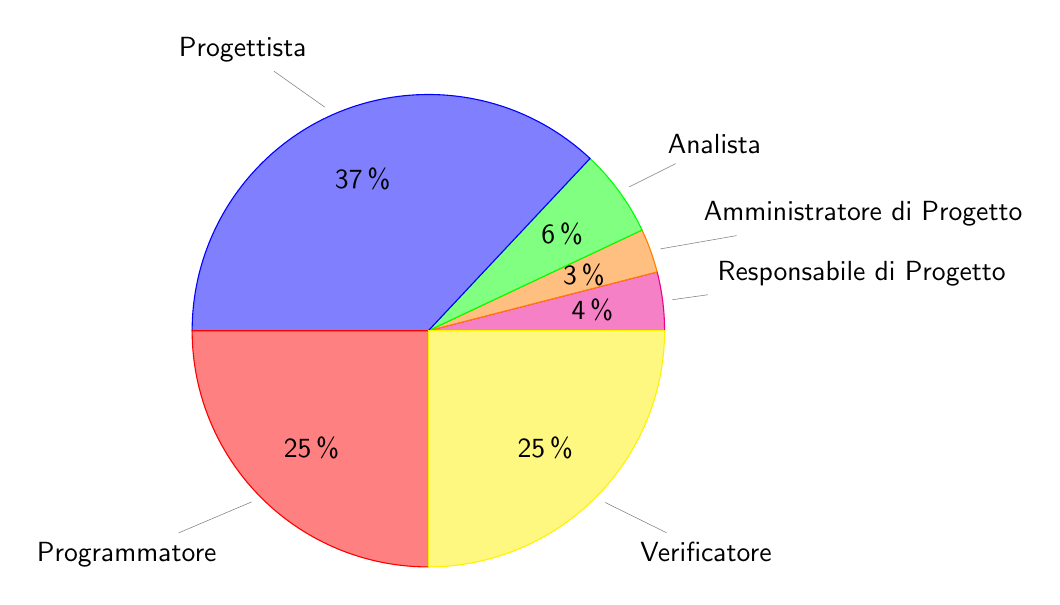
\begin{tikzpicture}[nodes = {font=\sffamily}]
	\foreach \percent/\name in {
		4/Responsabile di Progetto,
		3/Amministratore di Progetto,
		6/Analista,
		37/Progettista,
		25/Programmatore,
		25/Verificatore
	} {
	\ifx\percent\empty\else               % If \percent is empty, do nothing
	\global\advance\cyclecount by 1     % Advance cyclecount
	\global\advance\ind by 1            % Advance list index
	\ifnum5<\cyclecount                 % If cyclecount is larger than list
	\global\cyclecount=0              %   reset cyclecount and
	\global\ind=0                     %   reset list index
	\fi
	\pgfmathparse{\cyclelist[\the\ind]} % Get color from cycle list
	\edef\color{\pgfmathresult}         %   and store as \color
	% Draw angle and set labels
	\draw[fill={\color!50},draw={\color}] (0,0) -- (\angle:\radius)
	arc (\angle:\angle+\percent*3.6:\radius) -- cycle;
	\node at (\angle+0.5*\percent*3.6:0.7*\radius) {\percent\,\%};
	\node[pin=\angle+0.5*\percent*3.6:\name]
	at (\angle+0.5*\percent*3.6:\radius) {};
	\pgfmathparse{\angle+\percent*3.6}  % Advance angle
	\xdef\angle{\pgfmathresult}         %   and store in \angle
	\fi
};
\end{tikzpicture}
\caption{Costi rendicontati per ruoli}
\end{figure}

\subsubsection{Conclusioni}
Il costo totale per realizzare \PROGETTO{} evidenziato in tabella~\ref{tab2} e imputabile al proponente è di 11393 euro. Tale progetto richiede 630 ore di sviluppo ovvero un totale di ore 105 a componente, come illustrato precedentemente nella tabella~\ref{tab1}.

